% --------------------------------------------------------------
% This is all preamble stuff that you don't have to worry about.
% Head down to where it says "Start here"
% --------------------------------------------------------------
 
\documentclass[10pt]{article}
 
\usepackage[margin=.3in, voffset=.3in, ]{geometry} 
\usepackage{amsmath,amsthm,amssymb, mathtools}
\usepackage{multicol}
\usepackage[subnum]{cases}
\usepackage{relsize}
\usepackage[makeroom]{cancel}
\usepackage[english]{babel}
\usepackage{graphicx}
\usepackage{calligra}
\usepackage[normalem]{ulem}
\usepackage{caption}
\usepackage{subcaption}
\usepackage{fancyhdr}
\usepackage{mathrsfs}
\usepackage{bbold}
\usepackage{physics}
\usepackage{tikz}
\usepackage{vwcol}

\DeclareMathAlphabet{\mathcalligra}{T1}{calligra}{m}{n} 
\DeclareFontShape{T1}{calligra}{m}{n}{<->s*[2.2]callig15}{}


% Makes '\sr' make a script r
\newcommand{\sr}{\ensuremath{\mathcalligra{r}}}
 
\newcommand{\N}{\mathbb{N}}
\newcommand{\Z}{\mathbb{Z}}
\newcommand{\ihat}{\boldsymbol{\hat{\textbf{\i}}}}
\newcommand{\jhat}{\boldsymbol{\hat{\textbf{\j}}}}
\newcommand{\khat}{\boldsymbol{\hat{\textbf{k}}}}
\newcommand{\rhat}{\boldsymbol{\hat{\textbf{r}}}}
\newcommand{\srhat}{\boldsymbol{\hat{\textbf{\sr}}}}
\newcommand{\xhat}{\boldsymbol{\hat{\textbf{x}}}}
\newcommand{\yhat}{\boldsymbol{\hat{\textbf{y}}}}
\newcommand{\zhat}{\boldsymbol{\hat{\textbf{z}}}}
\newcommand{\nhat}{\boldsymbol{\hat{\textbf{n}}}}
\newcommand{\phihat}{\boldsymbol{\hat{\textbf{$\phi$}}}}
\newcommand{\thetahat}{\boldsymbol{\hat{\textbf{$\theta$}}}}
\newcommand{\rhohat}{\boldsymbol{\hat{\textbf{$\rho$}}}}

\newcommand{\ve}[1]{\boldsymbol{\mathbf{#1}}}
\newcommand{\vect}[1]{\boldsymbol{\mathbf{#1}}}
\newcommand{\vc}[1]{\mathbf{#1}}
\newcommand{\fracl}[2]{\mathlarger{\frac{#1}{#2}}}
%\newcommand{\dd}{\, \mathrm{d}}
\newcommand{\eo}{\epsilon_0}
\newcommand{\mo}{\mu_\circ}
\newcommand{\tder}[2]{\frac{\dd #1}{\dd #2}}
\newcommand{\pder}[2]{\frac{\partial #1}{\partial #2}}
\newcommand{\dtder}[2]{\frac{\dd^2 #1}{\dd #2^2}}
\newcommand{\ttder}[2]{\frac{\dd^3 #1}{\dd #2^3}}
\newcommand{\dpder}[2]{\frac{\partial^2 #1}{\partial #2^2}}
\newcommand{\tpder}[2]{\frac{\partial^3 #1}{\partial #2^3}}
\newcommand{\intas}{ \int_{-\infty}^\infty}
\newcommand{\wt}[1]{\widetilde{#1}}
%\newcommand{\ev}[1]{\left\langle #1 \right\rangle}
%\newcommand{\ket}[1]{\left| #1 \right\rangle}
%\newcommand{\bra}[1]{\left\langle #1 \right|}
%\newcommand{\braket}[2]{\left\langle #1 \right| \left. \! #2 \right\rangle}
\newcommand{\ce}{\wt{\vect{E}}}
\newcommand{\cb}{\wt{\vect{B}}}
\newcommand{\K}{\frac{1}{4 \pi \eo}}
\newcommand{\lrp}[1]{\left( #1 \right)}
\newcommand{\lrb}[1]{\left[ #1 \right]}
\newcommand{\lrc}[1]{\left\{ #1 \right\}}
\newcommand{\evalb}[1]{\left. #1 \right|}
\newcommand{\herm}[1]{#1^\dagger}
 
\newenvironment{theorem}[2][Theorem]{\begin{trivlist}
\item[\hskip \labelsep {\bfseries #1}\hskip \labelsep {\bfseries #2.}]}{\end{trivlist}}
\newenvironment{lemma}[2][Lemma]{\begin{trivlist}
\item[\hskip \labelsep {\bfseries #1}\hskip \labelsep {\bfseries #2.}]}{\end{trivlist}}
\newenvironment{exercise}[2][Exercise]{\begin{trivlist}
\item[\hskip \labelsep {\bfseries #1}\hskip \labelsep {\bfseries #2.}]}{\end{trivlist}}
\newenvironment{problem}[2][Problem]{\begin{trivlist}
\item[\hskip \labelsep {\bfseries #1}\hskip \labelsep {\bfseries #2.}]}{\end{trivlist}}
\newenvironment{question}[2][Question]{\begin{trivlist}
\item[\hskip \labelsep {\bfseries #1}\hskip \labelsep {\bfseries #2.}]}{\end{trivlist}}
\newenvironment{corollary}[2][Corollary]{\begin{trivlist}
\item[\hskip \labelsep {\bfseries #1}\hskip \labelsep {\bfseries #2.}]}{\end{trivlist}}


\newenvironment{Figure}
  {\par\medskip\noindent\minipage{\linewidth}}
  {\endminipage\par\medskip}

\pagenumbering{gobble}

\ifx\du\undefined
	\newlength{\du}
\fi
\setlength{\du}{15\unitlength}

\pagestyle{fancy}
\lhead{Thermodynamics Equations}
\chead{MSU Comprehensive Exam 2016}
\rhead{Roy Smart}


 
\begin{document}

\begin{multicols}{2}
	\tiny
	\setlength{\abovedisplayskip}{-25pt}
	\setlength{\belowdisplayskip}{-25pt}
	\setlength{\abovedisplayshortskip}{0pt}
	\setlength{\belowdisplayshortskip}{0pt}
	\begin{align*}
	& \small \hspace{-10pt} \textbf{Equilibrium and State Quantities} \small \\
	& \small \hspace{-10pt} \textbf{The Laws of Thermodynamics} \small \\	
	& \small \hspace{-10pt} \textbf{Phase Tranisitions and Chemical Reactions} \small \\
		& K(p,T) = \exp \lrc{\frac{1}{kT} \lrp{\sum_i a_i \mu_i(p,T) - \sum_j b_j \mu_j(p,T)}} = \frac{X_{B_1}^{b_1} X_{B_2}^{b_2}...}{X_{A_1}^{a_1} X_{A_2}^{a_2}...} \tag*{Law of mass action, determines concetration of species in chemical reaction (GNS 3.33)} \\
		& \frac{\Delta p}{p(T)} = X_{\text{sub}}	\tag*{Raoult's law, pressure of a solvent with dissolved material (GNS 3.39)} \\
		& X = X_0 \frac{p}{p_0}		\tag*{Henry-Dalton law, concentration of a gas in a solution (GNS pg. 78)} \\		






	\end{align*} \linebreak
	\setlength{\abovedisplayskip}{-25pt}
	\setlength{\belowdisplayskip}{-10pt}
	\setlength{\abovedisplayshortskip}{0pt}
	\setlength{\belowdisplayshortskip}{0pt}
	\begin{align*} 









	\end{align*}
	
	\begin{minipage}{0.3 \columnwidth}
		% Graphic for TeX using PGF
% Title: /home/byrdie/Diagram1.dia
% Creator: Dia v0.97.2
% CreationDate: Thu Jun 23 14:56:24 2016
% For: byrdie
% \usepackage{tikz}
% The following commands are not supported in PSTricks at present
% We define them conditionally, so when they are implemented,
% this pgf file will use them.
\ifx\du\undefined
  \newlength{\du}
\fi
\setlength{\du}{10\unitlength}
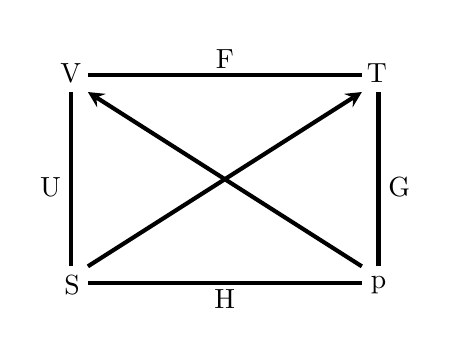
\begin{tikzpicture}
\pgftransformxscale{1.000000}
\pgftransformyscale{-1.000000}
\definecolor{dialinecolor}{rgb}{0.000000, 0.000000, 0.000000}
\pgfsetstrokecolor{dialinecolor}
\definecolor{dialinecolor}{rgb}{1.000000, 1.000000, 1.000000}
\pgfsetfillcolor{dialinecolor}
\definecolor{dialinecolor}{rgb}{1.000000, 1.000000, 1.000000}
\pgfsetfillcolor{dialinecolor}
\fill (29.350000\du,19.800000\du)--(29.350000\du,20.700000\du)--(29.860000\du,20.700000\du)--(29.860000\du,19.800000\du)--cycle;
\pgfsetlinewidth{0.100000\du}
\pgfsetdash{}{0pt}
\pgfsetdash{}{0pt}
\pgfsetmiterjoin
\definecolor{dialinecolor}{rgb}{1.000000, 1.000000, 1.000000}
\pgfsetstrokecolor{dialinecolor}
\draw (29.350000\du,19.800000\du)--(29.350000\du,20.700000\du)--(29.860000\du,20.700000\du)--(29.860000\du,19.800000\du)--cycle;
% setfont left to latex
\definecolor{dialinecolor}{rgb}{0.000000, 0.000000, 0.000000}
\pgfsetstrokecolor{dialinecolor}
\node at (29.605000\du,20.445000\du){p};
\definecolor{dialinecolor}{rgb}{1.000000, 1.000000, 1.000000}
\pgfsetfillcolor{dialinecolor}
\fill (29.600000\du,17.400000\du)--(29.600000\du,18.400000\du)--(30.600000\du,18.400000\du)--(30.600000\du,17.400000\du)--cycle;
\pgfsetlinewidth{0.100000\du}
\pgfsetdash{}{0pt}
\pgfsetdash{}{0pt}
\pgfsetmiterjoin
\definecolor{dialinecolor}{rgb}{1.000000, 1.000000, 1.000000}
\pgfsetstrokecolor{dialinecolor}
\draw (29.600000\du,17.400000\du)--(29.600000\du,18.400000\du)--(30.600000\du,18.400000\du)--(30.600000\du,17.400000\du)--cycle;
% setfont left to latex
\definecolor{dialinecolor}{rgb}{0.000000, 0.000000, 0.000000}
\pgfsetstrokecolor{dialinecolor}
\node at (30.100000\du,18.095000\du){G};
\definecolor{dialinecolor}{rgb}{1.000000, 1.000000, 1.000000}
\pgfsetfillcolor{dialinecolor}
\fill (29.300000\du,14.700000\du)--(29.300000\du,15.600000\du)--(29.827500\du,15.600000\du)--(29.827500\du,14.700000\du)--cycle;
\pgfsetlinewidth{0.100000\du}
\pgfsetdash{}{0pt}
\pgfsetdash{}{0pt}
\pgfsetmiterjoin
\definecolor{dialinecolor}{rgb}{1.000000, 1.000000, 1.000000}
\pgfsetstrokecolor{dialinecolor}
\draw (29.300000\du,14.700000\du)--(29.300000\du,15.600000\du)--(29.827500\du,15.600000\du)--(29.827500\du,14.700000\du)--cycle;
% setfont left to latex
\definecolor{dialinecolor}{rgb}{0.000000, 0.000000, 0.000000}
\pgfsetstrokecolor{dialinecolor}
\node at (29.563750\du,15.345000\du){T};
\definecolor{dialinecolor}{rgb}{1.000000, 1.000000, 1.000000}
\pgfsetfillcolor{dialinecolor}
\fill (21.900000\du,14.700000\du)--(21.900000\du,15.600000\du)--(22.480000\du,15.600000\du)--(22.480000\du,14.700000\du)--cycle;
\pgfsetlinewidth{0.100000\du}
\pgfsetdash{}{0pt}
\pgfsetdash{}{0pt}
\pgfsetmiterjoin
\definecolor{dialinecolor}{rgb}{1.000000, 1.000000, 1.000000}
\pgfsetstrokecolor{dialinecolor}
\draw (21.900000\du,14.700000\du)--(21.900000\du,15.600000\du)--(22.480000\du,15.600000\du)--(22.480000\du,14.700000\du)--cycle;
% setfont left to latex
\definecolor{dialinecolor}{rgb}{0.000000, 0.000000, 0.000000}
\pgfsetstrokecolor{dialinecolor}
\node at (22.190000\du,15.345000\du){V};
\definecolor{dialinecolor}{rgb}{1.000000, 1.000000, 1.000000}
\pgfsetfillcolor{dialinecolor}
\fill (21.950000\du,19.800000\du)--(21.950000\du,20.700000\du)--(22.487500\du,20.700000\du)--(22.487500\du,19.800000\du)--cycle;
\pgfsetlinewidth{0.100000\du}
\pgfsetdash{}{0pt}
\pgfsetdash{}{0pt}
\pgfsetmiterjoin
\definecolor{dialinecolor}{rgb}{1.000000, 1.000000, 1.000000}
\pgfsetstrokecolor{dialinecolor}
\draw (21.950000\du,19.800000\du)--(21.950000\du,20.700000\du)--(22.487500\du,20.700000\du)--(22.487500\du,19.800000\du)--cycle;
% setfont left to latex
\definecolor{dialinecolor}{rgb}{0.000000, 0.000000, 0.000000}
\pgfsetstrokecolor{dialinecolor}
\node at (22.218750\du,20.445000\du){S};
\definecolor{dialinecolor}{rgb}{1.000000, 1.000000, 1.000000}
\pgfsetfillcolor{dialinecolor}
\fill (21.200000\du,17.400000\du)--(21.200000\du,18.400000\du)--(22.200000\du,18.400000\du)--(22.200000\du,17.400000\du)--cycle;
\pgfsetlinewidth{0.100000\du}
\pgfsetdash{}{0pt}
\pgfsetdash{}{0pt}
\pgfsetmiterjoin
\definecolor{dialinecolor}{rgb}{1.000000, 1.000000, 1.000000}
\pgfsetstrokecolor{dialinecolor}
\draw (21.200000\du,17.400000\du)--(21.200000\du,18.400000\du)--(22.200000\du,18.400000\du)--(22.200000\du,17.400000\du)--cycle;
% setfont left to latex
\definecolor{dialinecolor}{rgb}{0.000000, 0.000000, 0.000000}
\pgfsetstrokecolor{dialinecolor}
\node at (21.700000\du,18.095000\du){U};
\definecolor{dialinecolor}{rgb}{1.000000, 1.000000, 1.000000}
\pgfsetfillcolor{dialinecolor}
\fill (25.400000\du,20.100000\du)--(25.400000\du,21.100000\du)--(26.400000\du,21.100000\du)--(26.400000\du,20.100000\du)--cycle;
\pgfsetlinewidth{0.100000\du}
\pgfsetdash{}{0pt}
\pgfsetdash{}{0pt}
\pgfsetmiterjoin
\definecolor{dialinecolor}{rgb}{1.000000, 1.000000, 1.000000}
\pgfsetstrokecolor{dialinecolor}
\draw (25.400000\du,20.100000\du)--(25.400000\du,21.100000\du)--(26.400000\du,21.100000\du)--(26.400000\du,20.100000\du)--cycle;
% setfont left to latex
\definecolor{dialinecolor}{rgb}{0.000000, 0.000000, 0.000000}
\pgfsetstrokecolor{dialinecolor}
\node at (25.900000\du,20.795000\du){H};
\definecolor{dialinecolor}{rgb}{1.000000, 1.000000, 1.000000}
\pgfsetfillcolor{dialinecolor}
\fill (25.400000\du,14.300000\du)--(25.400000\du,15.300000\du)--(26.400000\du,15.300000\du)--(26.400000\du,14.300000\du)--cycle;
\pgfsetlinewidth{0.100000\du}
\pgfsetdash{}{0pt}
\pgfsetdash{}{0pt}
\pgfsetmiterjoin
\definecolor{dialinecolor}{rgb}{1.000000, 1.000000, 1.000000}
\pgfsetstrokecolor{dialinecolor}
\draw (25.400000\du,14.300000\du)--(25.400000\du,15.300000\du)--(26.400000\du,15.300000\du)--(26.400000\du,14.300000\du)--cycle;
% setfont left to latex
\definecolor{dialinecolor}{rgb}{0.000000, 0.000000, 0.000000}
\pgfsetstrokecolor{dialinecolor}
\node at (25.900000\du,14.995000\du){F};
\pgfsetlinewidth{0.100000\du}
\pgfsetdash{}{0pt}
\pgfsetdash{}{0pt}
\pgfsetbuttcap
{
\definecolor{dialinecolor}{rgb}{0.000000, 0.000000, 0.000000}
\pgfsetfillcolor{dialinecolor}
% was here!!!
\definecolor{dialinecolor}{rgb}{0.000000, 0.000000, 0.000000}
\pgfsetstrokecolor{dialinecolor}
\draw (22.600000\du,20.400000\du)--(29.200000\du,20.400000\du);
}
\pgfsetlinewidth{0.100000\du}
\pgfsetdash{}{0pt}
\pgfsetdash{}{0pt}
\pgfsetbuttcap
{
\definecolor{dialinecolor}{rgb}{0.000000, 0.000000, 0.000000}
\pgfsetfillcolor{dialinecolor}
% was here!!!
\definecolor{dialinecolor}{rgb}{0.000000, 0.000000, 0.000000}
\pgfsetstrokecolor{dialinecolor}
\draw (22.200000\du,15.800000\du)--(22.200000\du,20.000000\du);
}
\pgfsetlinewidth{0.100000\du}
\pgfsetdash{}{0pt}
\pgfsetdash{}{0pt}
\pgfsetbuttcap
{
\definecolor{dialinecolor}{rgb}{0.000000, 0.000000, 0.000000}
\pgfsetfillcolor{dialinecolor}
% was here!!!
\definecolor{dialinecolor}{rgb}{0.000000, 0.000000, 0.000000}
\pgfsetstrokecolor{dialinecolor}
\draw (22.600000\du,15.400000\du)--(29.200000\du,15.400000\du);
}
\pgfsetlinewidth{0.100000\du}
\pgfsetdash{}{0pt}
\pgfsetdash{}{0pt}
\pgfsetbuttcap
{
\definecolor{dialinecolor}{rgb}{0.000000, 0.000000, 0.000000}
\pgfsetfillcolor{dialinecolor}
% was here!!!
\definecolor{dialinecolor}{rgb}{0.000000, 0.000000, 0.000000}
\pgfsetstrokecolor{dialinecolor}
\draw (29.600000\du,20.000000\du)--(29.600000\du,15.800000\du);
}
\pgfsetlinewidth{0.100000\du}
\pgfsetdash{}{0pt}
\pgfsetdash{}{0pt}
\pgfsetbuttcap
{
\definecolor{dialinecolor}{rgb}{0.000000, 0.000000, 0.000000}
\pgfsetfillcolor{dialinecolor}
% was here!!!
\pgfsetarrowsend{stealth}
\definecolor{dialinecolor}{rgb}{0.000000, 0.000000, 0.000000}
\pgfsetstrokecolor{dialinecolor}
\draw (22.600000\du,20.000000\du)--(29.200000\du,15.800000\du);
}
\pgfsetlinewidth{0.100000\du}
\pgfsetdash{}{0pt}
\pgfsetdash{}{0pt}
\pgfsetbuttcap
{
\definecolor{dialinecolor}{rgb}{0.000000, 0.000000, 0.000000}
\pgfsetfillcolor{dialinecolor}
% was here!!!
\pgfsetarrowsend{stealth}
\definecolor{dialinecolor}{rgb}{0.000000, 0.000000, 0.000000}
\pgfsetstrokecolor{dialinecolor}
\draw (29.200000\du,20.000000\du)--(22.600000\du,15.800000\du);
}
\end{tikzpicture}

	\end{minipage}
	\begin{minipage}{0.65 \columnwidth}
		\begin{itemize}
			\item The derivative of a potential (edge) with respect to a variable (corner) is given by the variable at the diagonally opposite corner. The arrows in the diagonals determine the sign. \\
			\item For the Maxwell relations, derivatives of variables along an edge of the quadrangle, at constant variable in the diagonally opposite corner, are just equal to the corresponding derivative on the other side.
		\end{itemize}
	\end{minipage}
	
	\setlength{\abovedisplayskip}{0pt}
	\setlength{\belowdisplayskip}{0pt}
	\setlength{\abovedisplayshortskip}{0pt}
	\setlength{\belowdisplayshortskip}{0pt}
	\begin{align*}
	& \small \hspace{-10pt} \textbf{Number of Microstates $\Omega$ and Entropy $S$} \small \\	
	& \small \hspace{-10pt} \textbf{Ensemble Theory and Microcanonical Ensembles} \small \\

	\end{align*} \newpage
	\setlength{\abovedisplayskip}{-25pt}
	\setlength{\belowdisplayskip}{-10pt}
	\setlength{\abovedisplayshortskip}{0pt}
	\setlength{\belowdisplayshortskip}{0pt}
	\begin{align*} 
	& \small \hspace{-10pt} \textbf{The Canonical Ensemble} \small \\

	& \small \hspace{-10pt} \textbf{Applications of Boltzmann Statistics} \small \\
		& \chi =N \frac{g^2 \mu_B^2 j(j+1)}{3kT} = \frac{C}{T}	\tag*{Magnetic susceptibility from the Curie law (GNS 8.52)} \\
		& C = Nk \lrp{\frac{2 \mu_B H}{kT}}^2 \exp \lrc{\frac{2 \mu_B H}{kT}} \lrp{1 + \exp\lrc{\frac{2 \mu_B H}{kT}}}^{-2}		\tag*{Schottky heat cap. (GNS 8.60)} \\
	& \small \hspace{-10pt} \textbf{The Macrocanonical Ensemble} \small \\

	\end{align*}
	
\end{multicols}
% --------------------------------------------------------------
%     You don't have to mess with anything below this line.
% --------------------------------------------------------------
 
\end{document}
